\section{Topologie de \texorpdfstring{$\mathbf{R}^{n}$}{Rn}}
\subsection{Boules de \texorpdfstring{$\mathbf{R}^{n}$}{Rn}}

Soit $\boldsymbol{x}\in \mathbf{R}^{n}$ et $\delta>0\in \mathbf{R}$:
\begin{definition}[Boule ouverte]
One definit une boule ouverte par l'ensemble
$$
B(\boldsymbol{x},\delta):= \{ \boldsymbol{z}\in \mathbf{R}^{n}:\lVert \boldsymbol{z}-\boldsymbol{x} \rVert <\delta \}
$$
\end{definition}
\begin{definition}[Boule fermee]
Une boule fermee est definit par l'ensemble
$$
\bar{B}(\boldsymbol{x},\delta):= \{ \boldsymbol{z}\in \mathbf{R}^{n}:\lVert \boldsymbol{z}-\boldsymbol{x} \rVert \leq\delta \}
$$
\end{definition}
\begin{definition}[Sphere]
Une sphere est defini par l'ensemble
$$
S(\boldsymbol{x},\delta):= \{ \boldsymbol{z}\in \mathbf{R}^{n}:\lVert \boldsymbol{z}-\boldsymbol{x} \rVert =\delta \}
$$
\end{definition}
\begin{definition}[Ensemble ouvert]
On dit que $E\subset \mathbf{R}^{n}$ est ouvert si 
$$
\forall \boldsymbol{x}\in E,\exists\delta>0:B(\boldsymbol{x},\delta)\subset E
$$
\end{definition}
\begin{definition}[Ensemble fermee]
On dit que $E\subset \mathbf{R}^{n}$ est ferme si son complement $$E^{C}=\mathbf{R}^{n}\setminus E:= \{ \boldsymbol{z}\in \mathbf{R}^{n}:\boldsymbol{z}\not\in E \}$$
est ouvert.
\end{definition}
\begin{definition}[Ensemble borne]
On dit que $E\subset \mathbf{R}^{n}$ est borne si
$$
\exists M>0:E\subset B(\boldsymbol{0},M)
$$
\end{definition}
\begin{exercise}
Montrer que:
\begin{itemize}
\item $B(\boldsymbol{x},\delta)$ est ouverte.
\item $\bar{B}(\boldsymbol{x},\delta)$ est fermee.
\end{itemize}
\end{exercise}

\subsection{Classification des points de \texorpdfstring{$\mathbf{R}^{n}$}{Rn} par rapport a \texorpdfstring{$E$}{E}}
\begin{example}
Soit 
$$
E=\{ (x_{1},x_{2})\in \mathbf{R}^{2}:x_{1}^{2}+x_{2}^{2}\ge 1,x_{1},x_{2}>0\}\cup \{ (0,0) \}
$$
\begin{figure}[h!]
\centering
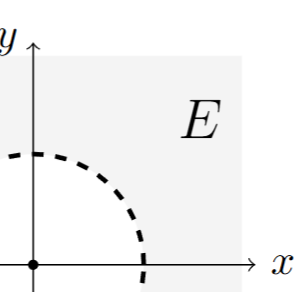
\includegraphics{points}
\end{figure}
on a dans les ensembles
$$
\mathring{E}=\{ (x_{1},x_{2})\in \mathbf{R}^{2}:x_{1}^{2}+x_{2}^{2}>1,x_{1},x_{2}>0 \}
$$
et
$$
\partial E=\{ x_{1}^{2}+x_{2}^{2}=1,x_{1}\ge0,x_{2}\ge 0 \}\cup \{ x_{1}=0,x_{2}\ge 1 \}\cup \{ x_{2}=0,x_{1}\ge 1 \}\cup \{ (0,0) \}
$$
et $\overline{E}=\mathring{E}\cup \partial E$.
\end{example}

On dit que $\boldsymbol{x}\in \mathbf{R}^{n}$ est:
\begin{itemize}
\item Un point interieuer de $E$ si $\exists\delta>0$ tel que $B(\boldsymbol{x},\delta)\subset E$. On appelle interieur de $E$ qu'on note par $\mathring{E}$ ou $\mathrm{int}(E)$ l'ensemble de ses points interieurs.
\item Un point frontiere de $E$ si $\forall\delta>0$ on a que $B(\boldsymbol{x},\delta)\cap E\neq \varnothing$ et $B(\boldsymbol{x},\delta)\cap E^{C}\neq\varnothing$. On appelle frontiere (ou bord) de $E$, note $\partial E$ l'ensemble de points frontiere de $E$. 
\item Un point adherant de $E$ si $\forall\delta>0$ on a que $B(\boldsymbol{x},\delta)\cap E\neq \varnothing$. Un point adherent est soit un point interieur, soit un point frontiere. On appelle adherence (ou fermeture) de $E$, note par $\overline{E}$ l'esnemble des points adherents de $E$. On a que $\overline{E}=\mathring{E}\cup \partial E=E\cup \partial E$. Un point adherent peut etre de deux types
\begin{itemize}
\item Un point isole si $\exists\delta>0$ tel que $B(\boldsymbol{x},\delta)\cap E=\{ \boldsymbol{x}\}$.
\item Un point d'accumulation si $\forall\delta>0$ on a $B(\boldsymbol{x},\delta)\cap E\setminus \{ x \}\neq \varnothing$
\end{itemize}
\end{itemize}

\subsection{Proprietes des ensembles ouverts}

\begin{itemize}
\item L'ensemble $\varnothing$ est ouvert par definition.
\item $\mathbf{R}^{n}$ est ouvert.
\item L'interieur $\mathring{E}$ est toujours ouvert.
\begin{proof}
Il faut demontrer que $\forall \boldsymbol{x}\in\mathring{E}$ il existe $\delta>0$ tel que $B(\boldsymbol{x},\delta)\subset\mathring{E}$. On sait que $\forall \boldsymbol{x}\in\mathring{E}$ il existe $\delta>0$ tel que $B(\boldsymbol{x},\delta)\subset E$ alors on doit verifier que $B(\boldsymbol{x},\delta)\subset\mathring{E}$. Pour tous $\boldsymbol{z}\in B(\boldsymbol{x},\delta)$ on a $B(\boldsymbol{z},\delta-\lVert \boldsymbol{z}-\boldsymbol{x} \rVert)\subset B(\boldsymbol{x},\delta)\subset E$ et donc $\boldsymbol{z}\in\mathring{E}$ et $B(\boldsymbol{x},\delta)\subset\mathring{E}$,
\end{proof}
\item $E$ est ouvert si et seulemnt si $E=\mathring{E}$.
\item L'union d'ouverts est ouverte.
\item L'union infinie denombrable d'ouverts est ouverte. On a $\{ E_{i} \}_{i\in \mathbf{N}}$ des $E_{i}$ ouverts alors $\bigcup _{i=1}^{\infty}E_{i}$ est ouverte.
\item L'intersection finie d'ouverts est ouverte.
\begin{proof}
Soient $\{ E_{i} \}_{i\in \mathbf{N}}$ ouverts et $F=\bigcap _{i=1}^{k}E_{i}$ et $\boldsymbol{x }\in F$ alors $\boldsymbol{x}\in E_{i}$ pour tous $i$ donc il existe $\delta _{i}>0$ tel que $B(\boldsymbol{x},\delta _{i})\subset E_{i}$ et $B(\boldsymbol{x},\min_{i=1,\dots,k})\subset F$ alors $F$ est ouvert.
\end{proof}
\begin{remark}
L'intersection infinie denombrable des $E_{i}$ ouverts n'est pas un ensemble ouvert. Comme contre-exemple on a $F=[0,1]$ et $E_{i}=(-1/i,1+1/i)$ dont l'intersection $\bigcap _{i=1}^{\infty}E_{i}=F$ qui est ferme.
\end{remark}
\end{itemize}

\subsection{Proprietes des ensembles fermes}
\begin{itemize}
\item $\mathbf{R}^{n}$ et $\varnothing$ sont fermes.
\item $\overline{E}$ est fermee.
\item $E$ est ferme si et seulement si $E=\overline{E}$.
\item L'intersection meme denombrable des fermes est fermee.
\item L'union finie de fermes est ferme. Comme contre-exemple soit $E_{i}=[1/i,1-1/i]$ alors $\bigcup _{i=2}^{\infty}E_{i}=(0,1)$.
\end{itemize}

\section{Caracterisation des ensembles fermes}

\begin{lemma}
Un ensemble $E\subset \mathbf{R}^{n}$ est ferme si et seulement si toute suite $\{ \boldsymbol{x}^{(k)} \}_{k\in \mathbf{N}}\subset E$ convergente, converge a $\boldsymbol{x}\in E$.
\end{lemma}
\begin{proof}

On montre le sens $\Rightarrow$: Si $E$ est ferme et $\{ \boldsymbol{x}^{(k)} \}_{k\in \mathbf{N}}\subset E$ est convergente a $\boldsymbol{x}\in \mathbf{R}^{n}$ implique que $\forall\delta>0$ on a que $B(\boldsymbol{x},\delta)\cap E\neq \varnothing$ donc $\boldsymbol{x}$ adhere a $E$ donc $\boldsymbol{x}\in \overline{E}$ et comme $\overline{E}=E$ alors $E$ est ferme. 

Sens $\Leftarrow$: Supposons que toute suite $\{ \boldsymbol{x}^{(k)} \}\subset E$ converge a $\boldsymbol{x}\in E$. Par l'absurde supposons que $E$ n'est pas ferme alors il existe $\boldsymbol{x}\in\bar{E}\setminus E$. Pour tout $\delta>0$ on a que $B(\boldsymbol{x},\delta)\cap E\neq \varnothing$,.Soit $\delta'=\frac{1}{k}$ alors $\boldsymbol{x}^{(k)}\in B(\boldsymbol{x},1/k)\cap E$ alors la suite $\{ \boldsymbol{x}^{(k)} \}\subset E$ mais on avait que $\boldsymbol{x}\in E^{C}$ donc on a une contradiction.
\end{proof}

\section{Ensembles compactes}
\begin{definition}\label{compact}
Un ensemble $E$ est compact si il est a la fois ferme et borne.
\end{definition}
\begin{theorem}
Un sous-ensemble $E\subset \mathbf{R}^{n}$ est compact (selon \ref{compact}) si et seulement si de toute suite $\{ \boldsymbol{x}^{(k)} \}_{k\in \mathbf{N}}\subset E$ on peut extraire une sous-suite convergente a un element $\boldsymbol{x}\in E$.
\end{theorem}
\begin{proof}
Sens $\Rightarrow$: Soit $E$ ferme et borne et $\{ \boldsymbol{x}^{(k)} \}_{k\in \mathbf{N}}\subset E$. En particulier $\{ \boldsymbol{x}^{(k)} \}$ est bornee donc par \ref{BW} on sait qu'il existe une sous-suite $\{ \boldsymbol{x}^{(k_{i})} \}_{i\in \mathbf{N}}\subset E$ convergente vers $\boldsymbol{x}\in \mathbf{R}^{n}$, puisque $E$ est femre alors $\boldsymbol{x}\in E$.
\end{proof}